%!TEX options = -shell-escape

\documentclass[12pt]{report}
\usepackage[a4paper,twoside,top=20mm,bottom=20mm,inner=30mm,outer=25mm]{geometry}
\usepackage[utf8]{inputenc}
\usepackage[greek,english]{babel}
\usepackage[scaled=0.86]{couriers}
\usepackage[toc,page,title,titletoc]{appendix}
\usepackage[pdfpagelabels,unicode]{hyperref}
\usepackage{bookmark}
\usepackage[fixlanguage]{babelbib}
\selectbiblanguage{greek}
\usepackage{titlesec}
\usepackage{etoolbox}
\usepackage{graphicx}
\usepackage{array}
\usepackage{amsmath}
\usepackage{minted}
\usepackage{subcaption}
\captionsetup{compatibility=false}
\graphicspath{ {images/} }
\usepackage[noend]{algpseudocode}
\usepackage{algorithm}
\usepackage{afterpage}
\usepackage{comment}
\usepackage{float}

\newcommand\blankpage{%
    \null
    \thispagestyle{empty}%
    \addtocounter{page}{-1}%
    \newpage}

\hypersetup{
  colorlinks=true,
  % linkcolor=green,
  citecolor=red,
  % filecolor=blue,
  urlcolor=blue,
  % pdftitle=,
  % pdfauthor=,
  % pdfsubject=,
  % pdfkeywords=
}

\setcounter{secnumdepth}{3}
\setcounter{tocdepth}{3}

\titleformat{\chapter}
  {\normalfont\LARGE\bfseries}{\thechapter}{1em}{}
\titlespacing*{\chapter}{0pt}{3.5ex plus 1ex minus .2ex}{2.3ex plus .2ex}

\makeatletter
\patchcmd\@resets@pp{%
  \def\Hy@chapapp{\appendixname }%
}{%
  \def\Hy@chapapp{appendix}%
}{}{\errmessage{Cannot patch \string\@resets@pp}}
\patchcmd\@resets@ppsub{%
  \def\Hy@chapapp{\appendixname }%
}{%
  \def\Hy@chapapp{appendix}%
}{}{\errmessage{Cannot patch \string\@resets@pp}}
\makeatother

\addto{\captionsgreek}{\renewcommand{\appendixpagename}{Παραρτήματα}}
\addto{\captionsgreek}{\renewcommand{\appendixtocname}{Παραρτήματα}}
\addto{\captionsgreek}{\renewcommand{\appendixname}{Παράρτημα}}

\begin{document}
\selectlanguage{greek}

\hypersetup{pageanchor=false}

\begin{titlepage}
  \centering
  
\includegraphics[width=0.15\textwidth]{pyrforos}\par\vspace{1cm}
  {\scshape\LARGE Εθνικό Μετσόβιο Πολυτεχνείο\\
  Σχολή Ηλεκτρολόγων Μηχανικών και Μηχανικών Η/Υ\par}
  \vspace{1cm}
  {\scshape\Large Εργασία στο Μεταπτυχιακό Μάθημα\\
  Διαχείριση Τεχνολογιών στο Ηλεκτρονικό Εμπόριο\par}
  \vspace{1.5cm}
  {\Large\bfseries Εγκατάσταση του Open-EDX και Δημιουργία Ενδεικτικού Μαθήματος\par}
  \vspace{2cm}
  {\large Δημήτριος Πολίτης (ΥΔ)\par}
  \vfill
  Επιβλέπων \par
  Καθ. Ευστάθιος Συκάς

  \vfill

% Bottom of the page
  {\large \today\par}
  \afterpage{\blankpage}
\end{titlepage}

\tableofcontents
\thispagestyle{empty}

\listoffigures
\thispagestyle{empty}

\begin{abstract}
Στο παρόν παρουσιάζεται η λειτουργία και η διαδικασία ανάπτυξης ενός μαθήματος στην πλατφόρμα \textlatin{Open-EDX}. Αρχικά  γίνεται αναφορά στην εν λόγω πλατφόρμα ηλεκτρονικής μάθησης και στη συνέχεια περιγράφεται αναλυτικά η διαδικασία εγκατάστασης της, με τη χρήση αυτοματοποιημένων εργαλείων (\textlatin{ansible, vagrant}). Τέλος περιγράφεται ο τρόπος δημιουργίας εντός τής πλατφόρμας, ενός ενδεικτικού μαθήματος. Η εργασία είναι διαθέσιμη από το σύνδεσμο \textlatin{\url{https://github.com/dpolitis/open-edx-install}}.

\vspace{10mm}

\noindent \textbf{Λέξεις κλειδιά:} Ηλεκτρονική Μάθηση, Ανοιχτός Κώδικας, Διαδίκτυο.
\end{abstract}

\hypersetup{pageanchor=true}
\clearpage
\pagenumbering{arabic}

\chapter{Εισαγωγή}\label{ch1}
\section{Εισαγωγή}
Η εποχή του Διαδικτύου επιβάλει την αναθεώρηση των παραδοσιακών τρόπων διεξαγωγής της διδασκαλίας μέσω φυσικής επαφής. Πλέον μεγάλο ποσοστό των μαθημάτων στην ακαδημαϊκή κοινότητα, πραγματοποιούνται με ηλεκτρονικά μέσα.

Η δημιουργία, η συντήρηση και η ανανέωση του περιεχομένου στις πλατφόρμες ηλεκτρονικής μαθησης αποτελεί σημαντικό παράγοντα στον κύκλο της μάθησης. Πλέον οι πλατφόρμες αυτές δεν περιορίζονται στην παροχή ηλεκτρονικών εγχειριδίων και σημειώσεων, αλλά αποτελούν πλέον εικονικές αίθουσες διδασκαλίας με τις δυνατότητες χρήσης \textlatin{live video streaming} ή \textlatin{avatar}.

\section{Ηλεκτρονική Μάθηση}
\subsection{Ορισμοί - Έννοιες}
Ηλεκτρονική Μάθηση ορίζεται ως η χρήση ηλεκτρονικών μέσων, εκπαιδευτικών τεχνολογιών αλλά και τεχνολογιών πληροφορίας και επικοινωνίας (ΤΠΕ) στην εκπαίδευση~\cite{wikipedia_2018_1}. Η ηλεκτρονική μάθηση διακρίνεται επιμέρους στη Σύγχρονη και Ασύγχρονη μάθηση.
  \paragraph{Σύγχρονη Mάθηση.} Ο όρος σύγχρονη μάθηση χρησιμοποιείται για να περιγράψει μορφές μάθησης και διδασκαλίας που λαμβάνουν χώρα την ίδια χρονική στιγμή, αλλά όχι στον ίδιο χώρο. Η Σύγχρονη μάθηση απαιτεί την ταυτόχρονη συμμετοχή του εκπαιδευτή και του εκπαιδευόμενου, όπου η αλληλεπίδραση μεταξύ των γίνεται σε πραγματικό χρόνο και οι συμμετέχοντες μπορούν να ανταλλάσσουν τόσο απόψεις όσο και εκπαιδευτικό υλικό. Η τηλεδιάσκεψη μέσω παγκόσμιου Ιστού, η τηλεδιάσκεψη μέσω βίντεο, οι συνομιλίες μέσω chat, η τηλεφωνία μέσω VoIP, η ζωντανή αναμετάδοση διαλέξεων με live streaming, τα online σεμινάρια (webinars) κ.α. όλα αποτελούν μορφές σύγχρονης μάθησης~\cite{moore_kearsley_2005}.
  \paragraph{Ασύγχρονη Μάθηση.} Ο όρος Ασύγχρονη μάθηση χρησιμοποιείται για να περιγράψει μορφές μάθησης και διδασκαλίας που λαμβάνουν χώρα τόσο σε διαφορετικές τοποθεσίες όσο και σε διαφορετικό χρόνο. Η Ασύγχρονη Εκπαίδευση δεν απαιτεί την ταυτόχρονη συμμετοχή του εκπαιδευτή και του εκπαιδευόμενου και οι συμμετέχοντες μπορούν να επιλέγουν μόνοι τους το προσωπικό τους εκπαιδευτικό χρονικό πλαίσιο και να συλλέγουν το εκπαιδευτικό υλικό σύμφωνα με αυτό. Το ηλεκτρονικό ταχυδρομείο, οι βιντεοδιασκέψεις, τα \textlatin{podcasts}, τα φόρουμ κ.α. αποτελούν μορφές ασύγχρονης μάθησης~\cite{stefan_hrastinski_2008}.

Η ασύγχρονη εκπαίδευση είναι περισσότερο ευέλικτη από την σύγχρονη. Στο είδος αυτό της εκπαίδευσης ανήκει η Αυτοδιδασκαλία, η Ημιαυτόνομη Εκπαίδευση και η Συνεργαζόμενη Εκπαίδευση~\cite{wikipedia_2018_1}.

\section{\textlatin{EdX}}
Το \textlatin{edX} είναι ένας πάροχος μαζικών ανοιχτών \textlatin{online} μαθημάτων (\textlatin{MOOC - massive open online course)}. Φιλοξενεί διαδικτυακά μαθήματα πανεπιστημιακού επιπέδου σε ένα ευρύ φάσμα επιστημονικών κλάδων, συμπεριλαμβανομένων και ορισμένων παρεχόμενων δωρεάν μαθημάτων. Διεξάγει επίσης έρευνα για τη μάθηση με βάση τον τρόπο με τον οποίο οι άνθρωποι χρησιμοποιούν την πλατφόρμα του. Είναι ένας μη κερδοσκοπικός οργανισμός και αξιοποιεί την πλατφόρμα ελεύθερου λογισμικού \textlatin{open edX}~\cite{edx_2018} για την παροχή των υπηρεσιών του.

Το Τεχνολογικό Ινστιτούτο της Μασαχουσέτης και το Πανεπιστήμιο του Χάρβαρντ δημιούργησαν το \textlatin{edX} τον Μάιο του 2012. Περισσότερα από 70 σχολεία, μη κερδοσκοπικοί οργανισμοί και επιχειρήσεις έκτοτε, προσφέρουν ή σχεδιάζουν να προσφέρουν, μαθήματα στον δικτυακό τόπο του \textlatin{edX}~\cite{edx_2019_1}. Από τις 29 Δεκεμβρίου 2017, η πλατφόρμα \textlatin{edX} έχει περίπου 14 εκατομμύρια φοιτητές που λαμβάνουν περισσότερα από 1.800 μαθήματα σε απευθείας σύνδεση~\cite{report_2018}.


\chapter{Το Λογισμικό \textlatin{Open edX}}\label{ch2}
\section{Γενικά Στοιχεία}
Το \textlatin{open edX} είναι το λογισμικό πλατφόρμας ανοιχτού κώδικα που αναπτύχθηκε από τo \textlatin{edX} και διατέθηκε ελεύθερα σε άλλα ιδρύματα τριτοβάθμιας εκπαίδευσης που επιθυμούν να παρέχουν παρόμοιες υπηρεσίες. Την 1η Ιουνίου 2013, το \textlatin{open edX} εξέδωσε ολόκληρο τον πηγαίο κώδικα της πλατφόρμα του υπό την άδεια \textlatin{GA GPLv3}. Ο παραπάνω πηγαίος κώδικας μπορεί να βρεθεί στο GitHub~\cite{edx_2019_2}.

Το λογισμικό εξυπηρετητή \textlatin{Open edX} είναι σχεδόν εξ' ολοκλήρου βασισμένο στη γλώσσα \textlatin{Python}, με το \textlatin{Django} ως \textlatin{web application framework}.

Αρκετά ιδρύματα τριτοβάθμιας εκπαίδευσης και διεθνείς οργανισμοί χρησιμοποιούν το \textlatin{open edX} για να παρέχουν υπηρεσίες \textlatin{MOOC}, όπως το \textlatin{MIT}~\cite{mit_open_learning_2018}, μέσω τη πλατφόρμας \textlatin{MITx} και το το Διεθνές Νομισματικό Ταμείο, το οποίο χρησιμοποιεί την πλατφόρμα \textlatin{open edX} για την πιλοτική κατάρτιση σε ηλεκτρονικά μαθήματα οικονομικών και χρηματοοικονομικών~\cite{edx_2014}.

Ορισμένες ιδιωτικές εταιρείες χρησιμοποιούν επίσης το λογισμικό \textlatin{open edX}, ώστε να παρέχουν εκπαίδευση στο προσωπικό τους και τους πελάτες τους. Για παράδειγμα, το \textlatin{MongoDB} χρησιμοποιεί το \textlatin Mongo University}, το οποίο στηρίζεται στο \textlatin{open edX}, για την παροχή εκπαίδευσης πάνω στο προϊόν της βάσης δεδομένων του~\cite{mongodb}.

\section{Συνοπτική Περιγραφή}
Το λογισμικό \textlatin{Open edX} αποτελείται από διάφορα επιμέρους τμήματα λογισμικού, το καθένα από τα οποία επιτελεί μια συγκεκριμένη εργασία. Όπου είναι δυνατόν, αυτά επικοινωνούν χρησιμοποιώντας σταθερά, τεκμηριωμένα API. Το κεντρικό στοιχείο της αρχιτεκτονικής του \textlatin{open edX} είναι το \textlatin{edx-platform}, το οποίο περιλαμβάνει τις εφαρμογές διαχείρισης μάθησης και συγγραφής μαθημάτων (\textlatin{LMS} και \textlatin{Studio}, αντίστοιχα). Αυτή η λειτουργικότητα υποστηρίζεται από μια συλλογή από άλλες αυτόνομες υπηρεσίες ιστού, οι οποίες ονομάζονται ανεξάρτητες εφαρμογές (\textlatin{Independently Deployed Applications - IDAs}). Ενδεικτικά, η αρχιτεκτονική της πλατφόρμας \textlatin{open edX} φαίνεται στο παρακάτω σχήμα~\ref{fig:edx_arch}:
\begin{figure}[h]
\centering
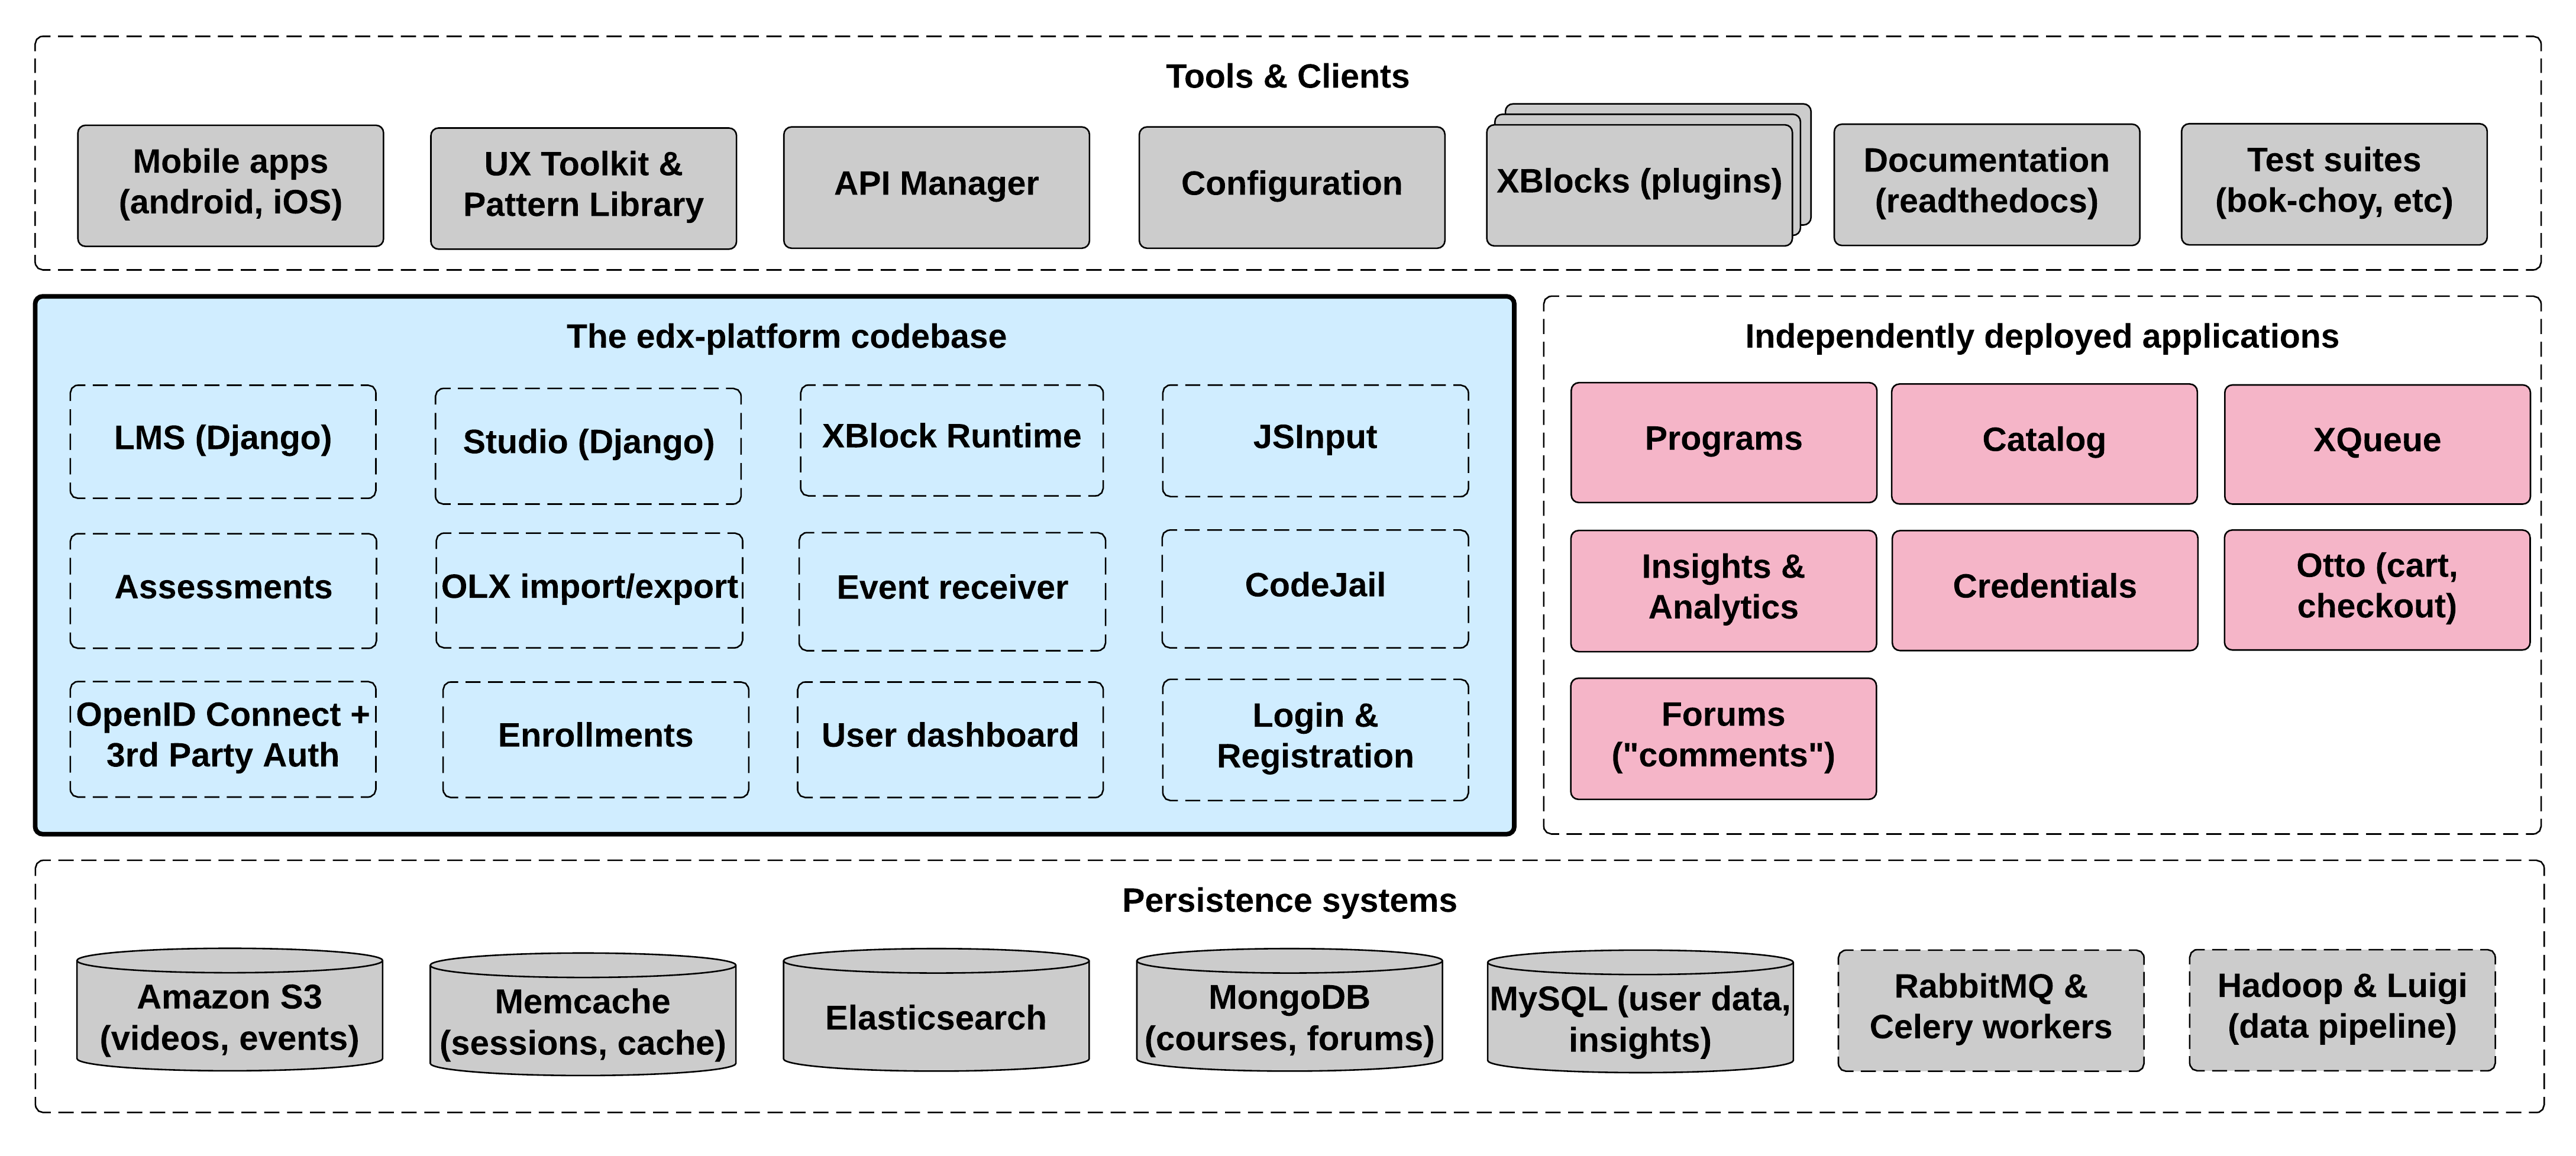
\includegraphics[width=0.8\textwidth, height=8cm]{edx-architecture}
\caption{Αρχιτεκονική Πλατφόρμας \textlatin{open edX}}
\label{fig:edx_arch}
\end{figure}

\section{Κύρια Μέρη}
\subsection{Σύστημα Διαχείρισης Μάθησης (\textlatin{LMS})}
Το \textlatin{LMS} είναι η διεπαφή του λογισμικού \textlatin{open edX}. Οι μαθητές παρακολουθούν μαθήματα χρησιμοποιώντας το \textlatin{LMS}. Το LMS παρέχει επίσης ένα πίνακα ελέγχου-ρυθμίσεων για τους διδάσκοντες στο οποίο οι χρήστες που έχουν το ρόλο διαχειριστή ή προσωπικού μπορούν να έχουν πρόσβαση επιλέγοντας το ρόλο του Εκπαιδευτή.

Το LMS χρησιμοποιεί έναν αριθμό αποθηκευτικών χώρων για το περιεχόμενο που διανέμει. Το περιεχόμενο των μαθημάτων αποθηκεύεται σε μια βάση \textlatin{MongoDB}, ενώ τα βίντεο είναι δυνατό να προβάλλονται από το \textlatin{YouTube} ή το \textlatin{Amazon S3}. Τα δεδομένα ανά εκπαιδευόμενο αποθηκεύονται σε μια βάση MySQL. Καθώς οι μαθητές μετακινούνται από μάθημα σε μάθημα και αλληλεπιδρούν με κάθε ένα από αυτά, τα δεδομένα που αφορούν σε αυτές τις αλληλεπιδράσεις συλλέγονται για περαιτέρω ανάλυση και εξαγωγή συμπερασμάτων.

Το \textlatin{LMS} αναλύεται περεταίρω στα παρακάτω επιμέρους τμήματα:
 \paragraph{Διεπαφή Χρήστη.} Ο κώδικας \textlatin{Django} από την πλευρά του εξυπηρετή χρησιμοποιεί το λογισμικό \textlatin{Mako} για τη παραγωγή διεπαφών και προτύπων (\textlatin{templates}). Ο κώδικας από την πλευρά του χρήστη είναι γραμμένος κυρίως σε \textlatin{JavaScript}, ενώ κάποια άλλα είναι γραμμένα σε \textlatin{Backbone.js framework}. Τα μέρη που χρησιμοποιούν \textlatin{CSS} υλοποιούνται με τη χρήση \textlatin{Bourbon - Sass frameworks}~\cite{edx_arch}.
 \paragraph{Περιήγηση Mαθημάτων.} Το λογισμικό \textlatin{open edX} παρέχει μια απλή πρώτη σελίδα για την περιήγηση εντός των παρεχόμενων μαθημάτων. Ο ιστότοπος \textlatin{\url{https://edx.org}} από την άλλη, έχει ξεχωριστή αρχική σελίδα και διαφορετική για την περιήγηση εντός των μαθημάτων, οι οποίες όμως δεν είναι ανοικτού κώδικα.
 \paragraph{Δομή μαθημάτων.} Τα μαθήματα στο \textlatin{open edX} αποτελούνται από μονάδες που ονομάζονται \textlatin{XBlocks}. Οι εκπαιδευτές μπορούν να γράψουν νέα \textlatin{XBlocks}, και με αυτό τον τρόπο να επεκτείνουν το σύνολο των βοηθημάτων για τα μαθήματά τους. Εκτός από τα \textlatin{XBlocks}, υπάρχουν και άλλοι τρόποι για να επεκταθεί η συμπεριφορά μαθημάτων:
\begin{itemize}
  \item Με τη χρήση εργαλείων \textlatin{LTI (Learning Tools Interoperability)}~\cite{lti}, για την ενσωματωση διαφόρων εργαλείων εκμάθησης σε ένα μάθημα \textlatin{οpen edX}.
  \item Με την ενσωμάτωση κώδικα \textlatin{Python}, για την παρουσίαση εκπαιδευτικών εργασιών - προβλημάτων και την αξιολόγηση των απαντήσεων των εκπαιδευομένων. Ο κώδικας σε αυτή την περίπτωση, εκτελείται σε ασφαλές περιβάλλον (\textlatin{CodeJail})~\cite{edx_arch}.
  \item Τμήματα κώδικα \textlatin{JavaScript} μπορούν να ενσωματωθούν με τη χρήση του \textlatin{JS Input}.
  \item Ολόκληρα μαθήματα μπορούν να εισαχθούν και να εξαχθούν με τη χρήση του \textlatin{OLX (open learning XML)}, ενός ειδικού φορμάτ για την περιγραφή μαθημάτων στο \textlatin{open-edX}.
\end{itemize}

\subsection{\textlatin{Studio}}
Το Studio είναι το περιβάλλον συγγραφής μαθημάτων. Οι εκπαιδευτές το χρησιμοποιούν για να δημιουργήσουν και να ενημερώσουν μαθήματα. Το \textlatin{Studio} γράφει τα μαθήματά του στην ίδια βάση δεδομένων \textlatin{Mongo} που χρησιμοποιεί το LMS.

\subsection{Συζητήσεις}
H λειτουργια των συζητήσεων για τα μαθήματα ελέγχεται από ένα \textlatin{IDA} που ονομάζεται \textlatin{comments} (ή \textlatin{forums}). Οι συζητήσεις είναι ένα από τα λίγα λειτουργικά μέρη του \textlatin{open edX} το οποίο δεν είναι γραμμένο σε γλώσσα \textlatin{Python}, αλλά σε \textlaint{Ruby} με τη χρήση του \textlatin{Sinatra framework}. Το \textlatin{LMS} χρησιμοποιεί ένα \textlatin{API}, το οποίο χρησιμοποιεί το \textlatin{comments service} για να ενσωματώσει τις συζητήσεις στην εμπειρία των μαθημάτων. Η υπηρεσία αυτή περιλαμβάνει μια διαδικασία κοινοποίησης, που στέλνει ειδοποιήσεις στους εγγεγραμμένους μαθητές, σχετικά με ενημερώσεις σε θέματα ενδιαφέροντος.

\subsection{Ενσωμάτωση Λειτουργικότητας Φορητών Συσκευών} Το \textlatin{open edX} περιλαμβάνει μια εφαρμογή για κινητά, διαθέσιμη για \textlatin{iOS} και \textlatin{Android}, η οποία επιτρέπει στους μαθητές να παρακολουθούν βίντεο-μαθήματα και πολλά άλλα. Το \textlatin{EdX} αναπτύσσει ενεργά την εφαρμογή για κινητά.

\subsection{Analytics}
Γεγονότα τα οποία περιγράφουν την αλληλεπίδραση των μαθητών, συλλέγονται από το \textlatin{analytics framework} του \textlatin{open edX}. Τα συμβάντα αποθηκεύονται ως \textlatin{JSON} σε \textlatin{S3}, υποβάλλονται σε επεξεργασία χρησιμοποιώντας εργαλεία \textlatin{Hadoop} και στη συνέχεια τα συγκεντρωτικά αποτελέσματα αποθηκεύονται στην \textlatin{MySQL}. Τα αποτελέσματα διατίθενται μέσω ενός \textlatin{REST API} στo \textlatin{Insights}, ένα \textlatin{IDA} που χρησιμοποιείται από τους εκπαιδευτές και τους διαχειριστές για τη διερεύνηση δεδομένων, τα οποία τους επιτρέπουν να γνωρίζουν τι κάνουν οι μαθητές τους και πώς χρησιμοποιούνται τα μαθήματά τους. Ένα διάγραμμα των στοιχείων και των τεχνολογιών που αποτελούν την αρχιτεκτονική του \textlatin{open edX analytics} φαίνεται στο παρακάτω σχήμα~\ref{fig:edx_analytics_arch}:
\begin{figure}[h]
\centering
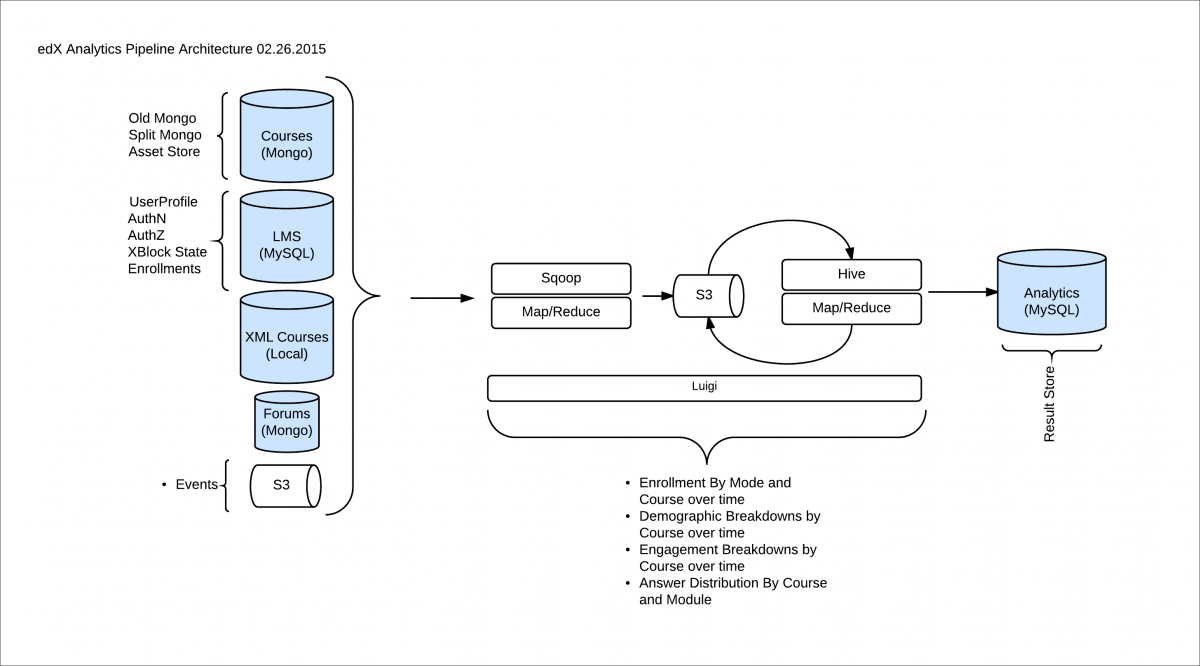
\includegraphics[width=0.8\textwidth, height=8cm]{edx-architecture-analytics}
\caption{Αρχιτεκονική \textlatin{open edX analytics}}
\label{fig:edx_analytics_arch}
\end{figure}

\subsection{Λειτουργίες Παρασκηνίου}
Ορισμένες εργασίες είναι αρκετά μεγάλες ώστε να εκτελούνται από από τις ίδιες τις εφαρμογές ιστού. Για αυτό το λόγο, τέτοιου είδους εργασίες ανατίθενται σε ξεχωριστές διεργασίες στο παρασκήνιο. Αυτές οι εργασίες τοποθετούνται σε ουρά και διανέμονται με τη βοήθεια των \textlatin{Celery} και \textlatin{RabbitMQ frameworks}. Παραδείγματα τέτοιων εργασιών περιλαμβάνουν:
\begin{itemize}
  \item Βαθμολόγηση μαθημάτων
  \item Αποστολή μαζικών μηνυμάτων ηλεκτρονικού ταχυδρομείου (με το \textlatin{Amazon SES})
  \item Δημιουργία αναφορών διανομής απαντήσεων
  \item Αποστολή πιστοποιητικών ολοκλήρωσης μαθημάτων
\end{itemize}

\subsection{Αναζήτηση}
Το \textlatin{open edX} χρησιμοποιεί το \textlatin{Elasticsearch} για αναζήτηση σε πολλαπλά επίπεδα, συμπεριλαμβανομένης της αναζήτησης εντός των μαθημάτων και των συζητήσεων.

\subsection{Επιπλέον Λειτουργικότητα}
Εκτός από τα όσα αναθέρθηκαν παραπάνω, το \textlatin{open edX} διαθέτει επίσης επιπλέον δυνατότητες, όπως τη διαχειρίση λειτουργιών ηλεκτρονικού εμπορίου~\cite{edx_arch}.

Το παρόν πραγματεύεται την ανάπτυξη ενός ενδεικτικού μαθήματος στην πλατφόρμα \textlatin{open edX}. Στα επόμενα παρουσιάζεται η διαδικασία εγκατάστασης της πλατφόρμας με τη χρήση αυτοματοποιημένων εργαλείων ανάπτυξης, ενώ γίνεται και μια συνοπτική αναφορά στα εργαλεία που χρησιμοποιήθηκαν κατά την εγκατάσταση.

\chapter{Εγκατάσταση της Πλατφόρμας \textlatin{open edX}}\label{ch3}
Για την εγκατάσταση της εν λόγω πλατφόρμας χρησιμοποιήθηκε αριθμός εργαλείων, τα οποία στην πλειονότητά τους βρίσκονται διαθέσιμα δωρεάν στο Διαδίκτυο (\textlatin{Open Source Software}). Στα επόμενα γίνεται μια σύντομη αναφορά στα εργαλεία που χρησιμοποιήθηκαν και στη διαδικασία της εγκατάστασης.

\section{\textlatin{\textlatin{Vagrant (Open Source VM Provissioner)}}}\label{vagrant}
Το \textlatin{Vagrant} είναι ένα εργαλείο δημιουργίας και διαχείρησης εικονικών μηχανών με τη χρήση μιας εξαιρετικά απλοποιημένης διαδικασίας~\cite{vagrant_by_hashicorp}. Το εργαλείο αυτό δίνει έμφαση στην αυτοματοποιημένη διαχείριση των εικονικών μηχανών και μειώνει σημαντικά το χρόνο δημιουργίας και παραμετροποίησης ενός \textlatin{development server}.

Είναι γραμμένο στη γλώσσα προγραμματισμού \textlatin{Ruby} και αποτελεί έναν ενιαίο τρόπο επικοινωνίας με δίάφορους \textlatin{providers} εικονικών μηχανών (όπως \textlatin{VirtualBox, VMware, AWS} κ.α.). Με τον τρόπο αυτό είναι δυνατή η δημιουργία εικονικών μηχανών με τις επιθυμητές παραμέτρους στον μικρότερο δυνατό χρόνο. Παράλληλα, για την εγκατάσταση πακέτων λογισμικού αλλά και παραμετροποίηση σε επίπεδο λειτουργικού συστήματος (ΛΣ), είναι δυνατή η συνεργασία με ευρέως διαδεδομένα \textlatin{provisioning tools}, όπως \textlatin{Chef, Puppet, Ansible} ακόμα και με απλά \textlatin{shell scripts}.

Το μεγαλύτερο ίσως πλεονέκτημα του υπόψη εργαλείου είναι η δυνατότητα παροχής στους προγραμματιστές ενός ενιαίου περιβάλλοντος, το οποίο είναι σταθερό και όσο κοντά γίνεται στο παραγωγικό εξυπηρετητή. Επίσης επειδή η παραμετροποίηση γίνεται με αυτόματο τρόπο, αφαιρείται από τους προγραμματιστές το βάρος της δημιουργίας, συντήρησης και αποσφαλμάτωσης του περιβάλλοντος ανάπτυξης.

Η αρχή λειτουργίας του \textlatin{Vagrant} στηρίζεται στην ύπαρξη μιας εικονικής μηχανής στελέχους (\textlatin{template/vagrant box}), η οποία είναι διαθέσιμη από τα επίσημα αποθετήρια \textlatin{\url{https://vagrantcloud.com/boxes/search}} είτε μπορεί να είναι δική μας. Κατόπιν μέσω μιας διαδικασίας κλωνοποίησης και εφαρμογής παραμέτρων, εντελώς διαφανούς για το χρήστη, αποδίδεται η εικονική μηχανή.

Όλα τα παραπάνω γίνονται με την εκτέλεση της εντολής \textlatin{\texttt{vagrant}} ακολουθούμενης από το αντίστοιχο \textlatin{switch}. Για παράδειγμα, η παρακάτω ακολουθία εντολών κατεβάζει μια εικονική μηχανή \textlatin{ubuntu 64bit} από το επίσημο αποθετήριο και την θέτει σε λειτουργία με τη βοήθεια του \textlatin{VirtualBox}.
\selectlanguage{english}
\begin{Verbatim}
  $ vagrant box add ubuntu/xenial64
  $ vagrant init
  $ vagrant up --provider=virtualbox
\end{Verbatim}
\selectlanguage{greek}
Για τη φιλοξενία του ιστοτόπου της εργασίας χρησιμοποιήθηκε μια μηχανή \textlatin{ubuntu 16.04 64bit} από το επίσημο αποθετήριο. Xρησιμοποιήθηκε ως \textlatin{Virtualization provider} το λογισμικό \textlatin{VirtualBox}. Στην συνέχεια με τη χρήση \textlatin{shell provissioner} έγινε η εγκατάσταση και παραμετροποίηση των απαραίτητων πακέτων και ρυθμίσεων του λειτουργικού συστήματος. Με τη χρήση του ίδιου \textlatin{provissioner}, μέσω της κλήσης του \textlatin{bash script} του Παραρτήματος~\ref{AppB} πραγματοποιήθηκαν τα τελικά στάδια εγκατάστασης και παραμετροποίησης της πλατφόρμας.

Όλα τα παραπάνω ορίζονται στο αρχείο \textlatin{\texttt{Vagrantfile}} το οποίο παρατίθεται στο Παράρτημα~\ref{AppA}.

\section{Εργαλείο Αυτοματοποίησης \textlatin{Ansible}}\label{ansible}
Το \textlatin{ansible} είναι open source software that automates software provisioning, configuration management, and application deployment~\cite{wikipedia_2019}. Ansible connects via SSH, remote PowerShell or via other remote APIs.

The name "Ansible" refers to a fictional instantaneous hyperspace communication system (as featured in Orson Scott Card's Ender's Game (1985),[9][10] and originally conceived by Ursula K. Le Guin for her novel Rocannon's World (1966))~\cite{worldcat}.

As with most configuration management software, Ansible has two types of servers: controlling machines and nodes. First, there is a single controlling machine which is where orchestration begins. Nodes are managed by a controlling machine over SSH. The controlling machine describes the location of nodes through its inventory.

To orchestrate nodes, Ansible deploys modules to nodes over SSH. Modules are temporarily stored in the nodes and communicate with the controlling machine through a JSON protocol over the standard output. When Ansible is not managing nodes, it does not consume resources because no daemons or programs are executing for Ansible in the background~\cite{wikipedia_2019}.

In contrast with popular configuration management software — such as Chef, Puppet, and CFEngine — Ansible uses an agentless architecture~\cite{wikipedia_2019}. With an agent-based architecture, nodes must have a locally installed daemon that communicates with a controlling machine. With an agentless architecture, nodes are not required to install and run background daemons to connect with a controlling machine. This type of architecture reduces the overhead on the network by preventing the nodes from polling the controlling machine~\cite{wikipedia_2019}.

\section{Διαδικασία Εγκατάστασης}
Μετά την εγκατάσταση της εικονικής μηχανής με τη χρήση του \textlatin{Vagrantfile}, όπως περιγράφηκε στο~\ref{vagrant}, ακολουθήθηκε η διαδικασία εγκατάστασης της πλατφόρμας με την κλήση του \textlatin{bash script} του Παραρτήματος~\ref{AppB}.

Οι γραμμές 61-71 του \textlatin{bash script} φροντίζουν ώστε .

Αρχικά υλοποιήθηκε το \textlatin{admin panel} με τι σελίδες διαχείρησης χρηστών και δικαιωμάτων. Στη συνέχεια υλοποιήθηκαν οι σελίδες \textlatin{login} για τους απλούς χρήστες και το \textlatin{admin panel}, ώστε να είναι έτοιμες για τα σενάρια αποσφαλμάτωσης. Έπειτα δημιουργήθηκε το αρχείο με τα μηνύματα της διεπαφής στα ελληνικά και τα αγγλικά, το οποίο εμπλουτίστηκε στη συνέχεια με νέο περιεχόμενο, κατά τη διαδικασία της ανάπτυξης.

Στα επόμενα στάδια δημιουργήθηκε η διεπαφή δημιουργίας μιας δημοπρασίας, με δυνατότητα ανάρτησης κειμένου, φωτογραφιών και άλλων πολυμέσων περιγραφής του προς πώληση προϊόντος. Τελευταία δημιουργήθηκε η διεπαφή πονταρίσματος (\textlatin{bidding}) με τις βασικές λειτουργίες αυτόματης ανανέωσης της σελίδας, λήξης της δημοπρασίας με χρονομέτρηση και ανάδειξη νικητή με βάση το ύψος της προσφοράς.

Με το πέρας της διαδικασίας ανάπτυξης δημιουργήθηκαν δοκιμαστικοί χρήστες και σενάρια δοκιμών για την αποσφαλμάτωση του κώδικα. Δοκιμάστηκαν πλήρη σενάρια και διορθώθηκαν σφάλματα, τα οποία είχαν να κάνουν με την μη σωστή αυτόματη ανανέωση του περιεχομένου της σελίδας.

\chapter{Δημιουργία Ενδεικτικού Μαθήματος}\label{ch4}
Στο παρόν γίνεται σύντομη αναφορά στη λειτουργικότητα της ιστοσελίδας δημοπρασιών που αναπτύχθηκε όπως στο~\ref{ch2}. Παρατίθενται \textlatin{screenshots} με επεξηγήσεις για τις κύριες λειτουργίες της σελίδας.

\section{Λειτουργικότητα Ιστοσελίδας}
\subsection{\textlatin{Admin Panel}}
Το πρώτο πράγμα που βλέπει κάποιος όταν επισκέπτεται την ιστοσελίδα είναι η φόρμα εισόδου. Για τις ανάγκες της εφαρμογής έχουν δημιουργηθεί δυο διαφορετικές σελίδες εισόδου. Μια για το \textlatin{admin panel} και μια για το \textlatin{login} των λοιπών χρηστών. Στην εικόνα~\ref{fig:login_1} παρουσιάζεται η σελίδα εισόδου στο \textlatin{admin panel}.
\begin{figure}[H]
\centering
\includegraphics[width=0.8\textwidth, height=8cm]{Screenshot-2018-1-14-login-e-auctions}
\caption{Φόρμα Εισόδου \textlatin{Admin Panel}}
\label{fig:login_1}
\end{figure}

Παρόμοια είναι και η σελίδα εισόδου χρηστών, αλλά είναι προσβάσιμη μέσω διαφορετικού \textlatin{url}. Μετά την επιτυχή είσοδο στη σελίδα του \textlatin{admin panel} ο διαχειριστής μπαίνει στη σελίδα διαχείρησης χρηστών του ιστοτόπου. Από εδώ είναι δυνατή η δημιουργία, διαγραφή και τροποποίηση των χρηστών της πλατφόρμας. Επίσης, είναι δυνατή η ανάθεση ρόλων (πωλητή, αγοραστή, παρατηρητή ή διαχειριστή) και η αλλαγή συνθηματικών. Η φόρμα διαχείρησης χρηστών εμφανίζεται στην εικόνα~\ref{fig:user_admin}.
\begin{figure}[H]
\centering
\includegraphics[width=0.8\textwidth, height=8cm]{Screenshot-2018-1-14-e-auctions-Admin-2}
\caption{Φόρμα Διαχείρησης Χρηστών}
\label{fig:user_admin}
\end{figure}

Στο επόμενο \textlatin{tab} εμφανίζονται τα εργαλεία της διαχείρισης όλων των δημοπρασιών (μόνο ακύρωση - διαγραφή, εικόνα~\ref{fig:auction_admin}).
\begin{figure}[H]
\centering
\includegraphics[width=0.8\textwidth, height=8cm]{Screenshot-2018-1-14-e-auctions-Admin-3}
\caption{Φόρμα Διαχείρησης Δημοπρασιών}
\label{fig:auction_admin}
\end{figure}

Το τελευταίο εργαλείο του \textlatin{admin panel} αφορά στη διαχείριση κατηγοριών προϊόντων. Εδώ καθορίζονται οι κατηγορίες στις οποίες καταχωρούνται τα προϊόντα κατά τη δημιουργία μιας δημοπρασίας. Είναι δυνατή η προσθήκη, διαγραφή και ενημέρωση της περιγραφής, του μοναδικού αναγνωριστικού και μιας προαιρετικής μικρογραφίας για την περιγραφή της κατηγορίας (εικόνα~\ref{fig:category_admin}).
\begin{figure}[H]
\centering
\includegraphics[width=0.8\textwidth, height=8cm]{Screenshot-2018-1-14-e-auctions-Admin-1}
\caption{Φόρμα Διαχείρησης Κατηγοριών Προϊόντων}
\label{fig:category_admin}
\end{figure}

\subsection{Λειτουργικότητα Δημοπρασιών}
Εάν ένας χρήστης με ιδιότητα πωλητή ή αγοραστή εισέλθει στο σύστημα με τα διαπιστευτήριά του, μπορεί αναλόγως το ρόλο που του έχει δοθεί στο \textlatin{admin panel}, να δημιουργήσει μια δημοπρασία ή να ποντάρει σε αυτή. Στην εικόνα~\ref{fig:auction_new} παρουσιάζεται μια από τις φόρμες του οδηγού καταχώρησης νέας δημοπρασίας από ένα πωλητή.
\begin{figure}[H]
\centering
\includegraphics[width=0.8\textwidth, height=8cm]{Screenshot-2018-1-14-Sell-e-auctions}
\caption{Φόρμα Καταχώρησης Δημοπρασιών}
\label{fig:auction_new}
\end{figure}

Όταν ο χρήστης έχει το ρόλο αγοραστή (\textlatin{bidder}) ή παρατηρητή (\textlatin{spectator}) μπορεί να έχει πρόσβαση στις σελίδες προόδου της δημοπρασίας, αλλά μπορεί να αλληλεπιδρά με αυτές και να ποντάρει μόνο εφόσον έχει το ρόλο του πωλητή. Στην εικόνα~\ref{fig:auction_bid} παρουσιάζεται μια από τις φόρμες του οδηγού καταχώρησης νέου "χτυπηματος" (\textlatin{bidding} δημοπρασίας από έναν αγοραστή.
\begin{figure}[H]
\centering
\includegraphics[width=0.8\textwidth, height=8cm]{Screenshot-2018-1-14-Essential-Phone-128-GB-Unlocked-with-Full-Display-Dual-Camera-Black-Moon-1}
\caption{Φόρμα Καταχώρησης Χτυπημάτων}
\label{fig:auction_bid}
\end{figure}

\section{Συμπεράσματα}
Στο παρόν, παρουσιάστηκε η διαδικασία ανάπτυξης καθώς και η λειτουργικότητα μιας ιστοσελίδας ηλεκτρονικών δημοπρασιών. Έγινε αναφορά σε βασικές έννοιες του ηλεκτρονικού εμπορίου και των ηλεκτρονικών δημοπρασιών. Στη συνέχεια περιγράφηκαν τα εργαλεία τα οποία χρησιμοποιήθηκαν για την ανάπτυξη του ιστοτόπου της εργασίας και ο τρόπος με τον οποίο αυτοματοποιήθηκαν και συνδυάστηκαν για την παραγωγή του τελικού αποτελέσματος, μετά και τη διαδικασία αποσφαλμάτωσης. Τέλος παρουσιάστηκαν οι βασικές λειτουργίες της σελίδας με συνοπτικό τρόπο και τη βοήθεια ανάλογων \textlatin{screenshots}.

Η ιστοσελίδα της εργασίας παρέχει πλήρη λειτουργικότητα διεξαγωγής των δημοπρασιών, με αυτόματη ανανέωση της σελίδας και ενημέρωση των χρηστών για την πορεία της διαδικασίας. Εκτός αυτού, με τη διάκριση των ρόλων των χρηστών και την ασφαλή αυθεντικοποίηση μέσω φορμών εισαγωγής στοιχείων, παρέχεται η απαιτούμενη διασφάλιση της διαδικασίας. Λειτουργικότητες που δεν ενσωματώθηκαν στην εργασία, όπως πληρωμές με τραπεζικές κάρτες, \textlatin{paypal} κ.α παραλήφθηκαν για λόγους κόστους, όπως αναλύθηκε στο~\ref{phpprobid}.

\begin{appendices}
\chapter{Αρχείο Ρύθμισης Εικονικής Μηχανής \textlatin{Vagrantfile}}\label{AppA}
\selectlanguage{english}
\inputminted[linenos, fontsize=\scriptsize, breaklines, baselinestretch=1]{ruby}{sources/Vagrantfile}
\selectlanguage{greek}
\chapter{\textlatin{Bash Script} Εγκατάστασης \textlatin{open edX}}\label{AppB}
\selectlanguage{english}
\inputminted[linenos, fontsize=\scriptsize, breaklines, baselinestretch=1]{bash}{sources/install_edx.sh}
\selectlanguage{greek}
\end{appendices}

\appendix

\bibliographystyle{babplain}
\bibliography{open-edx}

\end{document}